% !TeX root = main.tex
\section{数据分析}
\subsection{价格热力图}
通过对搜集到的数据进行回归分析与预测, 我们可以得到北京市与上海市的房价预测热力图, 如图 \ref{fig:predict} 所示.

\begin{figure}[H]
  \centering
  \subcaptionbox{北京市}{\includegraphics[width=.45\linewidth]{figures/beijing_predict.png}}
  \subcaptionbox{上海市}{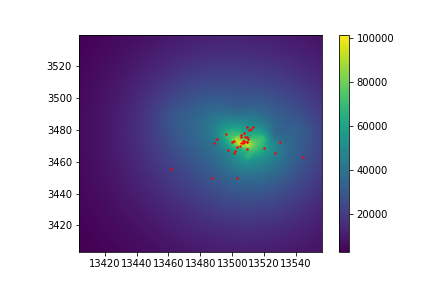
\includegraphics[width=.45\linewidth]{figures/shanghai_predict.png}}
  \caption{模型预测}
  \label{fig:predict}
\end{figure}

从预测图 (图 \ref{fig:predict}) 和样本分布 (图 \ref{fig:housing}) 的对比可以主观地发现二者的房价分布之间呈现出一致的趋势, 在北京市与上海市的中心均有显著的 10 万以上高房价的区域, 由内而外大致呈现递减的变化趋势.

值得注意的是, 在整张地图上, 市中心外存在多个高房价的区域, 离市中心的远近不是房价唯一的影响因素, 一个区域拥有商场, 医院, 公园等重要区位条件也是高房价的成因.

\subsection{区位分析}
在生成房价预测的同时, 通过回归分析同时可以得出各个区位因素的影响因子, 如图 \ref{fig:impact} 所示.

\begin{figure}[H]
  \centering
  \subcaptionbox{北京市}{\includegraphics[width=.45\linewidth]{figures/beijing_impact.png}}
  \subcaptionbox{上海市}{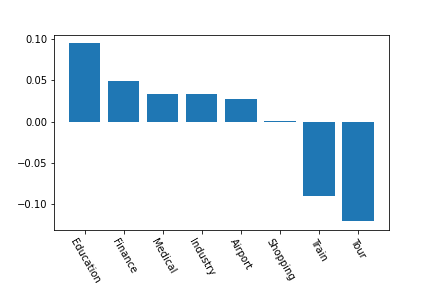
\includegraphics[width=.45\linewidth]{figures/shanghai_impact.png}}
  \caption{影响因子}
  \label{fig:impact}
\end{figure}

在北京与上海的对比中可以发现, 高居第一的都为 Incidents and Events.
此外, Tourist Attraction 的重要性也较大.
其他区位的影响因子具有一定的随机成分, 这是由于这些区位间并不独立:
例如, 由于市中心拥有良好的地理位置能够吸引足够大的人流量, 上海的景点 (豫园, 外滩等), 商业区 (淮海路, 南京路等) 同时多位于市中心区域, 那么这两个因素必然具有很大的相关性, 那么我们便难以排除这二者之间潜在的联系, 从而间接导致了区位排行的混乱性.

这是我们的模型的一大局限之处 --- 由于文化, 历史, 经济等多方面综合因素, 我们难以兼顾区位选择的完整性和独立性.

\subsection{模型评价}
\subsubsection{2018 年住房价格估测}
使用前文所述模型对北京市和上海市 2018 年的住房价格进行回归计算, 结果的判定系数 $R^2$ 分别为 \num{0.732} 与 \num{0.669}.
同时, 回归计算中也出现了异常偏大的条件数, 这意味着回归因子之间可能存在强相关性.
更加详细的计算结果见 \ref{sec:results} 部分.

我们用得到的模型对已有的数据回测, 得到误差分布如图 \ref{fig:test}.

\begin{figure}[H]
  \centering
  \includegraphics[width=.5\linewidth]{figures/test.png}
  \caption{误差分布}
  \label{fig:test}
\end{figure}

\subsubsection{2022 年住房价格估测}
在北京市随机选取灯市口, 西四, 五道口, 杨庄, 百子湾, 五个地点进行当前房价预测, 结果与出现了较大的误差, 在调查国家统计局数据后, 发现 2020 年的北京房价较 2018 年有 \SI{14}{\percent} 的上涨, 因此基于全北京房价均匀上涨的假设, 对数据进行了线性的校准, 得到结果如表 \ref{tab:predict_2022} 所示, 可以发现在预测 2022 年房价上也是较为可观的.

\begin{table}[H]
  \centering
  \caption{2022 年住房价格估测}
  \label{tab:predict_2022}
  \begin{tabular}{c|cccc}
    \toprule
    地区   & 2018 年房价 (估测)     & 2022 年房价 (估测)     & 2022 年房价 (样本) & 误差                  \\
    \midrule
    灯市口 & \tablenum{111743.1228} & \tablenum{127460.9104} & \tablenum{125000}  & \SI{1.97}{\percent}   \\
    西四   & \tablenum{119677.2265} & \tablenum{136511.0252} & \tablenum{151000}  & \SI{-9.60}{\percent}  \\
    五道口 & \tablenum{82661.68714} & \tablenum{94288.88005} & \tablenum{113000}  & \SI{-16.56}{\percent} \\
    杨庄   & \tablenum{57558.57881} & \tablenum{65654.76851} & \tablenum{53000}   & \SI{23.88}{\percent}  \\
    百子湾 & \tablenum{53822.89011} & \tablenum{61393.61783} & \tablenum{61000}   & \SI{0.65}{\percent}   \\
    \bottomrule
  \end{tabular}
\end{table}
